%\input{format}
%\begin{document}
%\input{BAB1}
\chapter{TEORI DASAR}\label{cha:teori}
%\AddToShipoutPicture{\BackgroundPic}
%\pagenumbering{arabic}

%%%%%%%%%%%%%%%%%%%%%%%%%%%%%%%%%%%%%%%%%%%%%%%%%%%%%%%%%%%%%%%

\section{Model Interaksi}\label{sec:modelinteraksi}
\hspace {0.5cm}Dalam melaksanakan tawaf gerak individu dapat dikaitkan dengan perilaku interaksi individual, karena bentuk kecepatan pergerakan orang pertama dalam melaksanakan tawaf bergantung dengan orang kedua didepannya dan orang didepannya tergantung dengan orang ketiga didepannya lagi dan seterusnya. Kita dapat meninjaunya dari segi fisika dengan mengasumsikan setiap individu adalah partikel. Partikel bergerak berkelompok karena kecepatan tetap dan arah setiap partikel resultan dari semua partikel berkelompok tersebut.

\hspace {0.5cm}Proses resultan dari partikel gerak individual menuju partikel yang berkelompok diakibatkan oleh perubahan variabel dalam sistem gaya yang mempengaruh.Variabel yang digunakan tersebut terletak pada order parameter. Orde parameter ini yang diterapkan kedalam dinamika \textit{flocking}.

% //revisi Penjelasan tentang flocking apa bagaimana dan penerapannya dulu%%%%%%%%%%%%%
\hspace {0.5cm}Istilah flocking digunakan untuk menjelaskan gerak berkelompok khususnya pada kawanan burung \citep{Toner1998}. Dimana setiap variabel dalam kawanan burung bergerak dengan arah dan kelajuan yang relatif sama tanpa saling bertabrakan satu sama lain.

%%%%%%%%%%%%%%%


\hspace {0.5cm}Dalam dinamika flocking yang dijalankan, terdapat \textit{input state} dan \textit{output state} yang digunakan dalam proses properti model partikel . Properti partikel ini berbentuk posisi, kecepatan, massa dan jarak gaya yang akan ditinjau dalam simulasi. Properti ini dalam \citep{Bajec2007} disebut dengan \textit{current state properties}  $q$. Yang dimaksud \textit{current state properties} adalah karakteristik yang dimiliki setiap partikel.
\begin{equation}
q = {p,\upsilon,z,m,\psi} 
\end{equation}



\section{Aplikasi gaya}\label{cha:aplikasi gaya}
\subsection{Flocking}\label{sec:flocking}

Mekanika Flocking berdasarkan reynolds mempunyai 3 gaya yang digunakan untuk membentuk kerumunan   \citep{Reynolds1987} \citep{Nasir2016}. Dimana hal ini dipakai oleh \citep{Chate2008} dalam modelnya \emph{boids model} untuk simulasi. Simulasi kerumunan akan terbentuk jika partikel bergerak sama dengan partikel sekitarnya, ,membentuk 1 titik area pemadatan partikel, dan mempunyai gaya pemisah agar partikel bergerak tanpa adanya partikel yang melekat/ tumbukan tidak elastis. Interaksi antar kerumunan ini dalam \citep{Chate2008} dinamakan SPP(\texttit{Self-Propelled Particles}). 

\begin{equation}
\vec{F}_i = \sum_{i \neq j} (\sum_{n=1}^{\infty} R_{n} \dfrac{\vec{P}_{ij}}{|\vec{P}_{ij}|^n}  + \sum_{n=1}^{\infty} I_{n} \dfrac{\vec{P}_{ij}}{|\vec{P}_{ij}|^n}). 
\end{equation}

\subsubsection{Alignment}\label{sec:alignment}
\hspace {0.5cm} Gaya Allignment digunakan untuk membuat partikel tetap bergerak satu grup. Berkaitan dengan sistem dalam tawaf, digunakan karena di dalam masjidil haram beberapa orang sering berkerumun untuk membentuk 1 grup agar tidak tersesat. Alasan lainnya, untuk penggunaan alignment ini membuat partikel menyamakan persepsi kecepatan dengan konsep yang terdepan akan mengurangi kecepatannya juga yang belakang akan menambah kecepatannya untuk berjalan bersamaan membentuk grup. secara matematika dapat ditulis sebagai berikut.

\begin{equation}
 F_i^a(p,q) = \alpha^a \dfrac{1}{N^c}\sum^{N^c}_{i \neq j}\dfrac{\vec{V}_{ji}}{|\vec{V}_{ji}|},\alpha^a = 1N
\end{equation}


\begin{figure}
\centering
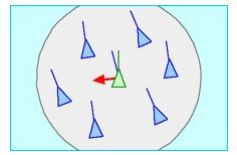
\includegraphics[scale=0.5]{gambar/allignment}
\caption{Bentuk Gerak Pensejajaran}
\end{figure}

\subsubsection{Cohesion}\label{sec:cohesion}
\hspace{0.5cm}Gaya kohesi digunakan untuk membuat partikel menarik tetangganya untuk berdekatan. Dimana posisi pusat dijadikan titik arah pergerakan sehingga partikel bergerak ke titik tersebut: berikut secara matematik dapat ditulis:

\begin{equation}
 F_i^k(p,q) = \alpha^k \dfrac{1}{N^c}\sum^{N^c}_{i \neq j}\dfrac{\vec{p}_{ji}}{|\vec{p}_{ji}|} , \alpha^k = 1N
\end{equation}
\begin{figure}
\centering
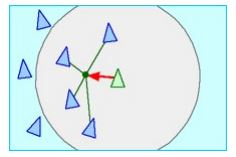
\includegraphics[scale=0.5]{gambar/cohesion}
\caption{Bentuk Gerak Pemusatan}
\end{figure}

\subsubsection{Separation}\label{sec:separation}
\hspace{0.5cm} Gaya separasi digunakan untuk partikel agar terjadi pemisahan dan meminimalisir pemisahan. Dalam konteks tawaf digunakan untuk menghindari seseorang menempal terhadap orang lain. dalam gaya separasi ini dilakukan variasi terhadap koefisiennya yaitu koefisien introversion atau tingkatjaga jarak dan tingkat racis untuk mengelompokkan jenis ras partikel berdasarkan warna.

\begin{equation}
 F_i^s(p,q) = \alpha^s \sum^{N^c}_{i \neq j}\dfrac{\vec{p}_{ji}}{|\vec{p}_{ji}|^2},\\
 \end{equation}
\begin{equation}
\alpha^a = radius + radius boids tetangga + koefisien introversion + koefisien racism
 \end{equation}

\begin{figure}
\centering
\includegraphics[scale=0.5]{gambar/separation}
\caption{Bentuk Gerak Pemisahan}
\end{figure}

\subsubsection{Circular Motion}\label{sec:circularmotion}
\hspace{0.5cm}Circular Motion atau bisa disebut gaya gerak memutar mengelilingi pusat gaya, dapat diaplikasikan kepada partikel yang bergerak secara flocking untuk membuat partikel seperti bergerak tawaf mengelilingi pusat gaya. Dimana pusat gaya berada di pusat kaaba berbentuk persegi. Gerak Flocking yang diterapkan perlu memenuhi syarat area tawaf. Dengan begitu gerak mengeliligi kaaba dapat berada di area dekat kaaba.

\[
  f(x)=\begin{cases}
    F_m^a(p,q) = \alpha^m \sum^{N^c}_{i \neq j}\dfrac{\vec{p}_{ji}}{|\vec{p}_{ji}|},\alpha^m = 1N , & \text{if x<50}.\\
    F_m^a(p,q) = \alpha^m \sum^{N^c}_{i \neq j}\dfrac{\vec{p}_{ji}}{|\vec{p}_{ji}|},\alpha^m = -1N, & \text{if x>50 and if x>300 }.
  \end{cases}
\]

\hspace{0.5cm}Pada persamaan pertama penerapan gaya menjauhi kaaba dengan syarat angka 50 jarak dari pusat kaaba sampai dinding. Sedangkan pada persamaan kedua penerapan gaya mendekati kaaba dengan asumsi partikel berada di luar area 50 sampai 300. Kedua gaya ini adalah gaya dominan yang diterapkan agar circular Motionnya bekerja.


\hspace{0.5cm}Penerapan gaya terbagi dalam 3 area,yaitu area dibagian luar putar,area dimana tawaf diterapkan dan area dinding kaaba. Pada bagian luar diterapkan gaya tarik menuju pusat, dibagian diding kaaba diterapkan gaya keluar untuk menjaga dinding kaaba. di area diterapkan gaya putar untuk partikel melakukan tawaf.


%%%%%%%%%%%%%%%%%%%%%%%%%%%%%%%%%%%%%%%%%%%%%%%%%%%%%%%%%%%%

\section{Model Partikel}\label{sec:modelpartikel}
\hspace {0.5cm}Model partikel sederhana dengan bentuk bulat menggambarkan partikel agent yang sedang bergerak
\begin{figure}
\centering
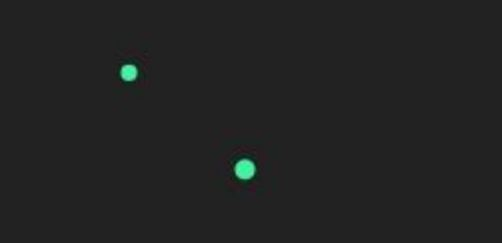
\includegraphics[scale=0.3]{gambar/ModelPartikel.JPG}
\caption{Model partikel sebagai titik posisi}
\end{figure}


\section{Model Ruang Partikel}\label{sec:ruangpartikel}

\hspace {0.5cm}Model ruang Partikel diformulasikan seperti gambar masjidil haram yang tertera pada gambar. Partikel bergerak berlawanan arah dengan ruang dibatasi boundary state yaitu dinding masjidil haram dan bagian dalam ada boundary state lagi berupa dinding kaaba. Akan tetapi dalam simulasi ini model ruang partikel dibatasi hanya pada kaaba dan area tawaf kaaba.
\begin{figure}
\centering
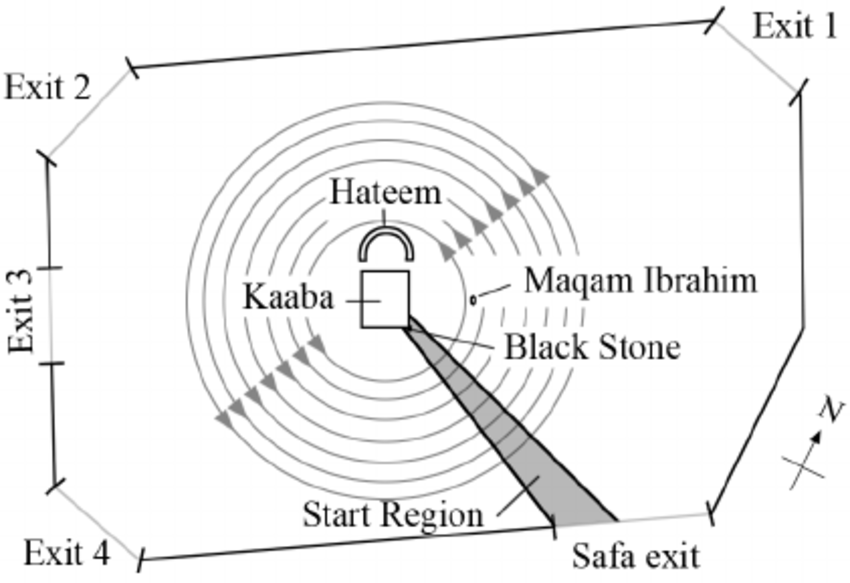
\includegraphics[scale=0.5]{gambar/layout2dmasjidilharam}
\caption{Model Area Masjidil Haram}
\end{figure}

\section{Persamaan Distribusi Normal }\label{sec:modelpartikel}
\hspace{0.5cm} Distribusi normal dalam program ini digunakan untuk menentukan nilai real dari koeffisien yang ada dalam nilai introversi, rasisme dan ketangkasan(quirkness). Hal ini mempengaruhi bentuk dari inisial tawaf yang akan terjadi, dalam kasus ini secara acak. 

\begin{equation}
f(x) =\dfrac{1}{\sigma \sqrt{2 \pi}} e^{-\dfrac{1}{2}(\dfrac{x-\mu}{\sigma})^2}
\end{equation}

\hspace{0.5cm} Normal distribusi penting digunakan dalam statistik karena sering digunakan untuk representasi nilai real dari variabel random yang distribusinya tidak diketahui\citep{Caseberg2009}. Pada simulasi ini distribusi normal digunaakan sebagai perbandingan untuk koefisien  partikel  agar dapat divariasikan.





\section{Metode Runge Kutta}\label{sec:metodeperhitungan}
\hspace{0.5cm} Metode Runge-Kutta adalah metode numerik yang banyak digunakan untuk menyelesaikan persamaan differensial. Metode ini adalah versi yang lebih kompleks dari metode euler yang banyak digunakan. Karena kompleksitasnya maka metode ini menawarkan grafik eksponensial yang lebih mendekati fungsi eksak.\\
Untuk fungsi y
\begin{equation}
\dfrac{dy}{dt} =f(y,t) , y(t_0)=y_0
\end{equation}

\begin{equation}
y_{n+1} = y_{n} + \dfrac{1}{6}h (k_1+2k_2+2k_3+k_4),
\end{equation}

\begin{equation}
Untuk n = 0,1,2,3,4 ......\\
\end{equation}
\begin{equation}
k_1 = f(y_{n} ,t_{n}),\\
\end{equation}
\begin{equation}
k_2 = f(y_{n}+h\dfrac{k_1}{2} ,t_{n}+\dfrac{h}{2}),\\
\end{equation}
\begin{equation}
k_3 = f(y_{n}+h\dfrac{k_2}{2} ,t_{n}+\dfrac{h}{2}),\\
\end{equation}
\begin{equation}
k_4 = f(y_{n}+hk_{1} ,t_{n}+h).\\
\end{equation}
\\
Untuk fungsi x
\begin{equation}
\dfrac{dx}{dt} =f(x,t) , x(t_0)=x_0
\end{equation}

\begin{equation}
x_{n+1} = x_{n} + \dfrac{1}{6}h (k_1+2k_2+2k_3+k_4),
\end{equation}

\begin{equation}
Untuk n = 0,1,2,3,4 ......
\end{equation}
\begin{equation}
k_1 = f(x_{n} ,t_{n}),
\end{equation}

\begin{equation}
k_2 = f(x_{n}+h\dfrac{k_1}{2} ,t_{n}+\dfrac{h}{2}),
\end{equation}

\begin{equation}
k_3 = f(x_{n}+h\dfrac{k_2}{2} ,t_{n}+\dfrac{h}{2}),
\end{equation}
\begin{equation}
k_4 = f(x_{n}+hk_{1} ,t_{n}+h).
\end{equation}


\begin{figure}

\centering
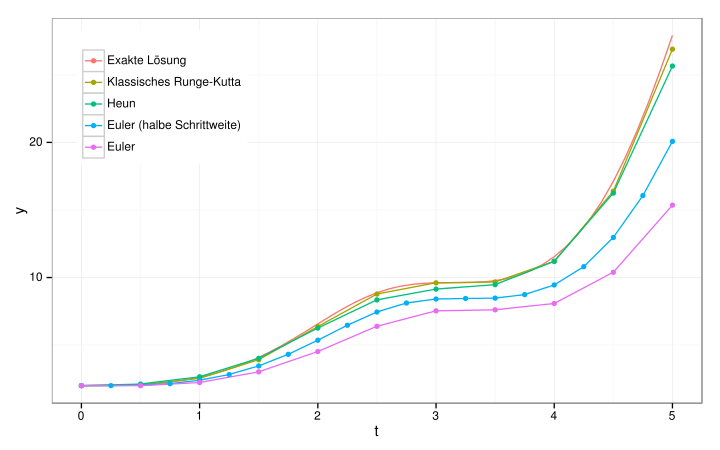
\includegraphics[scale=0.5]{gambar/comparison_euler}
\caption{Perbandingan euler dan runge-kutta}
\end{figure}

Dalam simulasi ini penggunaan runge-kutta digunakan karena alokasi memori komputer yang digunakan tidak terlalu besar. Metode ini juga dipertimbangkan dengan metode euler dimana tingkat error yang lebih rendah. Mempertimbangkan jumlah partikel yang digunakan maka diambil metode ini. Metode runge-kutta digunakan karena kinerja pada komputer ringan.



%\input{referensi}
%\end{document}